\documentclass[tikz, border=10pt]{standalone}
\usepackage{pgfplots}
\pgfplotsset{compat=1.18}
\usepackage{amsmath}

\begin{document}
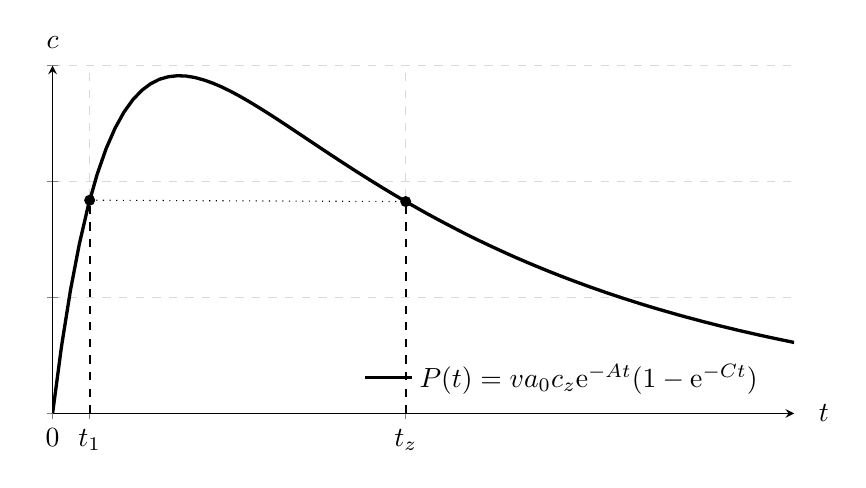
\begin{tikzpicture}
  % parametroj
  \pgfmathsetmacro{\vpar}{1}   % v
  \pgfmathsetmacro{\az}{1}     % a_0
  \pgfmathsetmacro{\cz}{10}    % c_z
  \pgfmathsetmacro{\A}{0.5}    % malkreska koef. A
  \pgfmathsetmacro{\C}{2.5}    % kreska koef. C

  % punktoj kaj valoroj en t0 kaj tz
  \pgfmathsetmacro{\tzero}{0.21}
  \pgfmathsetmacro{\ttz}{2.0}
  \pgfmathsetmacro{\Pzero}{\vpar * \az * \cz * exp(-\A * \tzero) * (1 - exp(-\C * \tzero))}
  \pgfmathsetmacro{\Ptz}{\vpar * \az * \cz * exp(-\A * \ttz) * (1 - exp(-\C * \ttz))}

  \begin{axis}[
    width=11cm,
    height=6cm,
    axis lines=left,
    xlabel={$t$},
    ylabel={$c$},
    xlabel style={at={(ticklabel* cs:1.02)}, anchor=west},
    ylabel style={at={(ticklabel* cs:1.02)}, anchor=south, rotate=-90},
    xmin=0, xmax=4.2,
    ymin=0, ymax=6,
    xtick={0, \tzero, \ttz},
    xticklabels={0, $t_1$, $t_z$}, 
    ytick={},
    yticklabels={}, 
    grid=major,
    grid style={dashed, gray!30},
    samples=100, 
    domain=0:5,
    legend pos=south east,
    % --- stilo de legendo ---
    legend style={
      fill=none,   
      draw=none
    }    
  ]

    % funkcio: P(t)=v a_0 c_z\mathrm{e}^{-At}(1-\mathrm{e}^{-Ct})
    \addplot[black, very thick] {\vpar * \az * \cz * exp(-\A * x) * (1 - exp(-\C * x))};
    \addlegendentry{$P(t) = v a_0 c_z\mathrm{e}^{-At}(1-\mathrm{e}^{-Ct})$}

    % vertikaloj en t0 kaj tz
    \draw[black, dashed, thick] (axis cs:\tzero, 0) -- (axis cs:\tzero, \Pzero);
    \draw[black, dashed, thick] (axis cs:\ttz,   0) -- (axis cs:\ttz,   \Ptz);

    \draw[black, dotted, thin] (axis cs:\tzero,   \Pzero) -- (axis cs:\ttz, \Ptz);


    % funkcivaoloroj tie kiel punktoj
    \fill[black] (axis cs:\tzero, \Pzero) circle (2pt);
    \fill[black] (axis cs:\ttz,   \Ptz)   circle (2pt);

    % asimptoto ĉe c = c_z
    %\addplot[black, dashed, thick] {\cz};
    %\addlegendentry{limvaloro $c_z$}

  \end{axis}
\end{tikzpicture}
\end{document}